\scanpage{118}
Supposons maintenant que $(r_\nu)$ soit la suite des
modules des zéros d'une fonction entière $f(z)$.
On aura $\displaystyle 2\pi n(r)\unsure{:|=}\int_0^{\deleted{\unsure{a}}2\pi}\frac{f'(re^{i\varphi})}{f(re^{i\varphi})}re^{i\varphi}\,d\varphi$, d'où
\[
\begin{aligned}
2\pi\int_a^b n(r)\mu(r)\,dr
&=\int_a^b\int_0^{2\pi}\frac{f'(re^{i\varphi})}{f(re^{i\varphi})}e^{i\varphi}\cdot\deleted{d\varphi}\ r\mu(r)\,dr\,d\varphi\\
&=\int_0^{2\pi}d\varphi\int_a^b
\underset{d_r\log f(re^{i\varphi})}{\underset{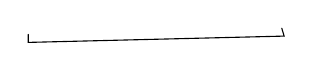
\begin{tikzpicture}[x=1cm,y=1cm,baseline=(current bounding box.center),line cap=round]\draw (0,.1)--(0,0)--(3.25,.08)--(3.22,.18);\end{tikzpicture}}{\frac{f'(re^{i\varphi})}{f(re^{i\varphi})}e^{i\varphi}\,dr}}\ (r\mu(r))
\end{aligned}
\]
\[
\int_a^b=\left[r\mu(r)\log f(re^{i\varphi})\right]_a^b-\int_a^b\log f(re^{i\varphi})\,d(r\mu(r))
\]
(en supposant $\mu(r)$ continûment différentiable)

-- On choisit brutalement la détermination
principale du logarithme -- pas de trou-\newline
ble, car les intégrales \deleted{\unsure{si elles ont|simplement}} doubles
qui interviennent sont convergentes)
\figure{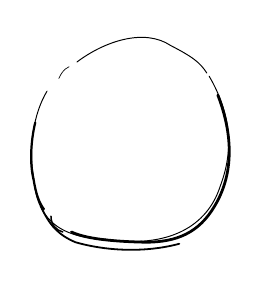
\begin{tikzpicture}[x=.01cm,y=-.01cm,line cap=round,line join=round]
\draw[line width=.35pt] (77,51) .. controls (113,24) and (163,8) .. (196,30) .. controls (223,44) and (233,51) .. (242,65);
\draw[line width=.25pt] (67,57) .. controls (60,60) and (56,67) .. (54,72);
\draw[line width=.35pt] (39,88) .. controls (22,116) and (15,160) .. (22,197) .. controls (25,248) and (52,274) .. (112,276) .. controls (194,289) and (243,259) .. (259,209) .. controls (278,159) and (271,114) .. (245,69);
\draw[line width=.8pt] (24,128) .. controls (18,153) and (17,181) .. (22,201) .. controls (25,219) and (29,230) .. (35,238);
\draw[line width=1pt] (256,93) .. controls (276,145) and (276,194) .. (252,234) .. controls (232,268) and (204,280) .. (164,280) .. controls (118,279) and (87,275) .. (70,267);
\draw[line width=.65pt] (31,234) .. controls (42,259) and (54,271) .. (75,280) .. controls (117,292) and (166,293) .. (207,282);
\draw[line width=.55pt] (44,247) .. controls (44,258) and (51,265) .. (59,267);
\end{tikzpicture}}
D'où, en substituant, intervertissant les signes $\int\!\int$, et
\margin{en prenant les parties réelles}
\[
\hbox{\begingroup\setbox0=\hbox{$\displaystyle \displaystyle \deleted{2\pi}\int_{\unsure{a}}^b n(r)\mu(r)\,dr\unsure{:|=}\left[r\mu(r)V(r)\right]_a^b-\int_a^b V(r)\,d(r\mu(r))$}\kern5pt\rlap{\tikz[baseline=0pt]{\draw[line width=.35pt] (-4pt,\the\dimexpr\ht0+4pt\relax)--(\the\dimexpr\wd0+5pt\relax,\the\dimexpr\ht0+4pt\relax);\draw[line width=.4pt] (-5pt,\the\dimexpr\ht0+1pt\relax)--(-4pt,\the\dimexpr-\dp0-1pt\relax);\draw[line width=.4pt] (-4pt,\the\dimexpr-\dp0-3pt\relax)--(-4pt,\the\dimexpr-\dp0-4pt\relax)--(-1pt,\the\dimexpr-\dp0-4pt\relax);\draw[line width=.35pt] (1pt,\the\dimexpr-\dp0-4pt\relax)--(\the\dimexpr\wd0+2pt\relax,\the\dimexpr-\dp0-4pt\relax);\draw[line width=.35pt] (\the\dimexpr\wd0+5pt\relax,\the\dimexpr\ht0+1pt\relax)--(\the\dimexpr\wd0+5pt\relax,\the\dimexpr-\dp0-1pt\relax);}}\copy0\kern6pt\endgroup}
\]
où \qquad \uline{$\displaystyle V(r)=\frac1{2\pi}\int_0^{2\pi}\log|f(re^{i\varphi}\unsure{\vert|)}\,d\varphi$}
Prenons $\mu(r)=-\lambda'(r)$, on obtient \enspace $(0<a<b<+\infty$
\[
\hbox{\begingroup\setbox0=\hbox{$\displaystyle \begin{aligned}
\sum_{\substack{\nu\unsure{,}\\a<r_\nu<b}}\lambda(r_\nu)^{\deleted{\unsure{\alpha}}}
&=\lambda^{\unsure{\mathord{-}|'}}(b)n(b-0)-\lambda(a)n(a+0)+[r\mu(r)V(r)]_a^b\deleted{\unsure{+\int^b V(r)\,d(r\mu|+\int^b}}\\
&\qquad+\int_a^b V(r)\,d(r\lambda'(r))
\end{aligned}$}\kern5pt\rlap{\tikz[baseline=0pt]{\draw[line width=.35pt] (-4pt,\the\dimexpr\ht0+4pt\relax)--(\the\dimexpr\wd0+5pt\relax,\the\dimexpr\ht0+4pt\relax);\draw[line width=.4pt] (-5pt,\the\dimexpr\ht0+1pt\relax)--(-4pt,\the\dimexpr-\dp0-1pt\relax);\draw[line width=.35pt] (-1pt,\the\dimexpr-\dp0-4pt\relax)--(\the\dimexpr\wd0+2pt\relax,\the\dimexpr-\dp0-4pt\relax);\draw[line width=.4pt] (\the\dimexpr\wd0+5pt\relax,\the\dimexpr-\dp0+5pt\relax)--(\the\dimexpr\wd0+5pt\relax,\the\dimexpr-\dp0-4pt\relax);}}\copy0\kern6pt\endgroup}
\]
\margin{119}
